\begin{frame}{Սահմանումներ և նշանակումներ}
\begin{itemize}
    \item Դիտարկվում են ոչ կողմնորոշված \textbf{գրաֆներ} (առանց պատիկ կողերի և օղակների) և \textbf{մուլտիգրաֆներ} (պատիկ կողեր թույլատրվում են),
    \item $V(G)$-ով և $E(G)$-ով կնշանակենք, համապատասխանաբար, $G$ գրաֆի (մուլտիգրաֆի) \textbf{գագաթների} և \textbf{կողերի} բազմությունները,
    \item $d_G(v)$-ն $v$ գագաթի \textbf{աստիճանն} է,
    \item $\delta(G)$-ն և $\Delta(G)$-ն, համապատասխանաբար, \textbf{նվազագույն և առավելագույն աստիճաններն} են,
    \item $diam(G)$-ն $G$ գրաֆի (մուլտիգրաֆի) \textbf{տրամագիծն} է:
\end{itemize} 
\end{frame}

\begin{frame}{Ճիշտ կողային ներկումներ}
\begin{columns}
\begin{column}{0.5\textwidth}
\begin{itemize}
    \item $\alpha : E(G) \rightarrow \mathbb{N}$ ֆունկցիան կոչվում է $G$ մուլտիգրաֆի \textbf{ճիշտ կողային ներկում}, եթե $\forall v \in V(G)$ գագաթին կից կողերը ներկված են զույգ առ զույգ տարբեր գույներով:
    \item<2-> $S(v,\alpha)$-ով նշանակում ենք $v$ գագաթի \textbf{սպեկտրը}՝ $v$-ին կից կողերի գույների բազմությունը:
    \item<2-> $\underline{S}(v, \alpha) = \min{S(v,\alpha)}$:
    \item<2-> $\overline{S}(v, \alpha) = \max{S(v,\alpha)}$:
\end{itemize}
\end{column}
\begin{column}{0.5\textwidth}
    \begin{figure}[t!]
    \centering
    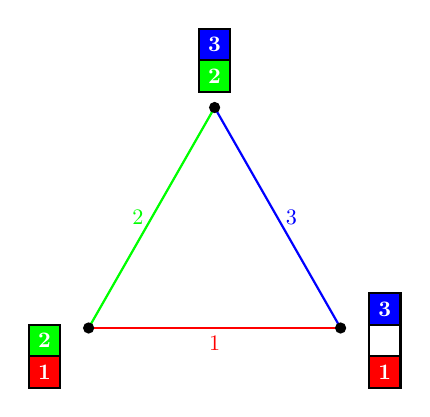
\begin{tikzpicture}[style=thick,scale=0.8, every node/.style={scale=0.8}]
        \coordinate (V1) at (0cm,0cm);
        \coordinate (V2) at (4cm,0cm);
        \coordinate (V3) at (2cm,3.5cm);
        
        \draw (V1) edge[red, thick] node[below]{$1$} (V2);
        \draw (V2) edge[blue, thick] node[right]{$3$} (V3);
        \draw (V1) edge[green, thick] node[left]{$2$} (V3);
        
        \draw[fill=black] (V1) circle (2pt) ;
        \draw[fill=black] (V2) circle (2pt) ;
        \draw[fill=black] (V3) circle (2pt) ;
        
        
        \node<2->[draw,fill=red,text=white,minimum height=0.5cm,minimum width=0.5cm] at (-0.7cm,-0.7cm) {$\mathbf{1}$};
        \node<2->[draw,fill=green,text=white,minimum height=0.5cm,minimum width=0.5cm] at (-0.7cm,-0.2cm) {$\mathbf{2}$};
        
        \node<2->[draw,fill=red,text=white,minimum height=0.5cm,minimum width=0.5cm] at (4.7cm,-0.7cm) {$\mathbf{1}$};
        \node<2->[draw,fill=white,text=white,minimum height=0.5cm,minimum width=0.5cm] at (4.7cm,-0.2cm) {$\mathbf{2}$};
        \node<2->[draw,fill=blue,text=white,minimum height=0.5cm,minimum width=0.5cm] at (4.7cm,0.3cm) {$\mathbf{3}$};
        
        
        \node<2->[draw,fill=green,text=white,minimum height=0.5cm,minimum width=0.5cm] at (2cm,4cm) {$\mathbf{2}$};
        \node<2->[draw,fill=blue,text=white,minimum height=0.5cm,minimum width=0.5cm] at (2cm,4.5cm) {$\mathbf{3}$};
    \end{tikzpicture}
    \end{figure}
\end{column}
\end{columns}
\end{frame}


\begin{frame}{Ճիշտ կողային ներկումներ}
\begin{columns}
\begin{column}{0.6\textwidth}
\begin{itemize}
    \item $G$ մուլտիգրաֆի \textbf{քրոմատիկ դասը}՝ $\chi'(G)$, ճիշտ կողային ներկումներում անհրաժեշտ գույների նվազագույն քանակն է:
    \item $\chi'(G)$-ն որոշելը NP-լրիվ խնդիր է:
\end{itemize}
\begin{theorem}[Վիզինգ, 1965]
$\Delta(G) \leq \chi'(G) \leq \Delta(G) + \mu(G)$,\\
որտեղ $\mu(G)$-ն $G$-ում կողերի առավելագույն պատիկությունն է:
\end{theorem}
\end{column}
\begin{column}{0.4\textwidth}
    
\begin{figure}[t!]
    \centering
    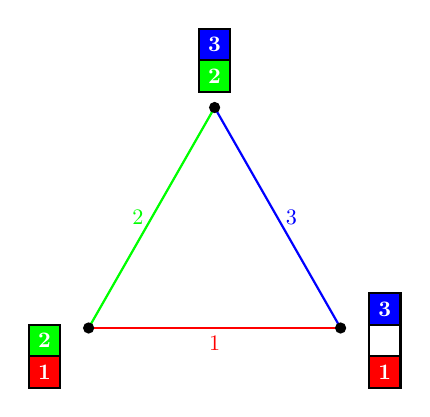
\begin{tikzpicture}[style=thick,scale=0.8, every node/.style={scale=0.8}]
        \coordinate (V1) at (0cm,0cm);
        \coordinate (V2) at (4cm,0cm);
        \coordinate (V3) at (2cm,3.5cm);
        
        \draw (V1) edge[red, thick] node[below]{$1$} (V2);
        \draw (V2) edge[blue, thick] node[right]{$3$} (V3);
        \draw (V1) edge[green, thick] node[left]{$2$} (V3);
        
        \draw[fill=black] (V1) circle (2pt) ;
        \draw[fill=black] (V2) circle (2pt) ;
        \draw[fill=black] (V3) circle (2pt) ;
        
        
        \node[draw,fill=red,text=white,minimum height=0.5cm,minimum width=0.5cm] at (-0.7cm,-0.7cm) {$\mathbf{1}$};
        \node[draw,fill=green,text=white,minimum height=0.5cm,minimum width=0.5cm] at (-0.7cm,-0.2cm) {$\mathbf{2}$};
        
        \node[draw,fill=red,text=white,minimum height=0.5cm,minimum width=0.5cm] at (4.7cm,-0.7cm) {$\mathbf{1}$};
        \node[draw,fill=white,text=white,minimum height=0.5cm,minimum width=0.5cm] at (4.7cm,-0.2cm) {$\mathbf{2}$};
        \node[draw,fill=blue,text=white,minimum height=0.5cm,minimum width=0.5cm] at (4.7cm,0.3cm) {$\mathbf{3}$};
        
        
        \node[draw,fill=green,text=white,minimum height=0.5cm,minimum width=0.5cm] at (2cm,4cm) {$\mathbf{2}$};
        \node[draw,fill=blue,text=white,minimum height=0.5cm,minimum width=0.5cm] at (2cm,4.5cm) {$\mathbf{3}$};
    \end{tikzpicture}
    \end{figure}
\end{column}
\end{columns}
\end{frame}

\begin{frame}{Միջակայքային ներկումներ}
\begin{columns}
\begin{column}{0.6\textwidth}
\begin{itemize}
    \item $\alpha: E(G) \rightarrow \{1,\ldots,t\}$ ճիշտ կողային ներկումը կանվանենք միջակայքային կողային $t$-ներկում, եթե ցանկացած $v \in V(G)$ գագաթի սպեկտրը միջակայք է:
    \item Միջակայքային ներկելի մուլտիգրաֆների բազմությունը նշանակում ենք $\mathfrak{N}$-ով:
    \item Երբ $G \in \mathfrak{N}$, $w(G)$-ն և $W(G)$-ն $t$-ի, համապատասխանաբար, փոքրագույն և մեծագույն արժեքներն են, որոնց համար $G$-ն ունի միջակայքային $t$-ներկում:
\end{itemize}

\end{column}
\begin{column}{0.4\textwidth}
\begin{figure}[t!]
    \centering
    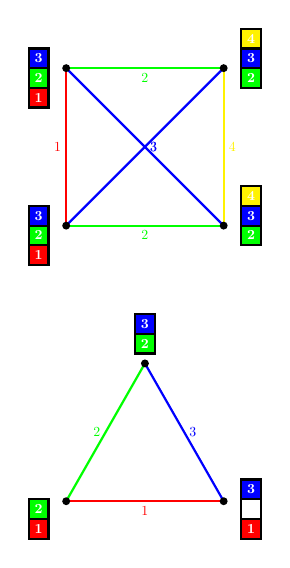
\begin{tikzpicture}[style=thick,scale=0.5, every node/.style={scale=0.5}]
    %% K4
        \coordinate (u1) at (0cm,7cm);
        \coordinate (u2) at (4cm,7cm);
        \coordinate (u3) at (4cm,11cm);
        \coordinate (u4) at (0cm,11cm);
        
        \draw (u1) edge[green, thick] node[below]{$2$} (u2);
        \draw (u3) edge[green, thick] node[below]{$2$} (u4);
        \draw (u1) edge[blue, thick] node[right]{$3$} (u3);
        \draw (u2) edge[blue, thick] node[right]{$3$} (u4);
        \draw (u1) edge[red, thick] node[left]{$1$} (u4);
        \draw (u2) edge[yellow, thick] node[right]{$4$} (u3);
        
        \draw[fill=black] (u1) circle (2pt) ;
        \draw[fill=black] (u2) circle (2pt) ;
        \draw[fill=black] (u3) circle (2pt) ;
        \draw[fill=black] (u4) circle (2pt) ;
        
        
        \node[draw,fill=red,text=white,minimum height=0.5cm,minimum width=0.5cm] at (-0.7cm,6.25cm) {$\mathbf{1}$};
        \node[draw,fill=green,text=white,minimum height=0.5cm,minimum width=0.5cm] at (-0.7cm,6.75cm) {$\mathbf{2}$};
        \node[draw,fill=blue,text=white,minimum height=0.5cm,minimum width=0.5cm] at (-0.7cm,7.25cm) {$\mathbf{3}$};
%         \node[draw,fill=yellow,text=white,minimum height=0.5cm,minimum width=0.5cm] at (-0.7cm,7.75cm) {$\mathbf{4}$};
        
%         \node[draw,fill=red,text=white,minimum height=0.5cm,minimum width=0.5cm] at (4.7cm,6.25cm) {$\mathbf{1}$};
        \node[draw,fill=green,text=white,minimum height=0.5cm,minimum width=0.5cm] at (4.7cm,6.75cm) {$\mathbf{2}$};
        \node[draw,fill=blue,text=white,minimum height=0.5cm,minimum width=0.5cm] at (4.7cm,7.25cm) {$\mathbf{3}$};
        \node[draw,fill=yellow,text=white,minimum height=0.5cm,minimum width=0.5cm] at (4.7cm,7.75cm) {$\mathbf{4}$};
    
    	\node[draw,fill=red,text=white,minimum height=0.5cm,minimum width=0.5cm] at (-0.7cm,10.25cm) {$\mathbf{1}$};
        \node[draw,fill=green,text=white,minimum height=0.5cm,minimum width=0.5cm] at (-0.7cm,10.75cm) {$\mathbf{2}$};
        \node[draw,fill=blue,text=white,minimum height=0.5cm,minimum width=0.5cm] at (-0.7cm,11.25cm) {$\mathbf{3}$};
%         \node[draw,fill=yellow,text=white,minimum height=0.5cm,minimum width=0.5cm] at (-0.7cm,7.75cm) {$\mathbf{4}$};
        
%         \node[draw,fill=red,text=white,minimum height=0.5cm,minimum width=0.5cm] at (4.7cm,6.25cm) {$\mathbf{1}$};
        \node[draw,fill=green,text=white,minimum height=0.5cm,minimum width=0.5cm] at (4.7cm,10.75cm) {$\mathbf{2}$};
        \node[draw,fill=blue,text=white,minimum height=0.5cm,minimum width=0.5cm] at (4.7cm,11.25cm) {$\mathbf{3}$};
        \node[draw,fill=yellow,text=white,minimum height=0.5cm,minimum width=0.5cm] at (4.7cm,11.75cm) {$\mathbf{4}$};
    
    %% TRIANGLE
        \coordinate (V1) at (0cm,0cm);
        \coordinate (V2) at (4cm,0cm);
        \coordinate (V3) at (2cm,3.5cm);
        
        \draw (V1) edge[red, thick] node[below]{$1$} (V2);
        \draw (V2) edge[blue, thick] node[right]{$3$} (V3);
        \draw (V1) edge[green, thick] node[left]{$2$} (V3);
        
        \draw[fill=black] (V1) circle (2pt) ;
        \draw[fill=black] (V2) circle (2pt) ;
        \draw[fill=black] (V3) circle (2pt) ;
        
        
        \node[draw,fill=red,text=white,minimum height=0.5cm,minimum width=0.5cm] at (-0.7cm,-0.7cm) {$\mathbf{1}$};
        \node[draw,fill=green,text=white,minimum height=0.5cm,minimum width=0.5cm] at (-0.7cm,-0.2cm) {$\mathbf{2}$};
        
        \node[draw,fill=red,text=white,minimum height=0.5cm,minimum width=0.5cm] at (4.7cm,-0.7cm) {$\mathbf{1}$};
        \node[draw,fill=white,text=white,minimum height=0.5cm,minimum width=0.5cm] at (4.7cm,-0.2cm) {$\mathbf{2}$};
        \node[draw,fill=blue,text=white,minimum height=0.5cm,minimum width=0.5cm] at (4.7cm,0.3cm) {$\mathbf{3}$};
        
        
        \node[draw,fill=green,text=white,minimum height=0.5cm,minimum width=0.5cm] at (2cm,4cm) {$\mathbf{2}$};
        \node[draw,fill=blue,text=white,minimum height=0.5cm,minimum width=0.5cm] at (2cm,4.5cm) {$\mathbf{3}$};
    \end{tikzpicture}
    \end{figure}
    
\end{column}
\end{columns}
\end{frame}
